\section{Evaluation}

To evaluate the performance of the colocating scheduler in comparison to other schedulers, we conduct a series of experiments focusing on overall CPU and memory usage that are critical for assessing scheduler efficiency and effectiveness. These metrics can reflect how well a scheduler performs under various loads and conditions.

Hereby, we design experiments that can simulate cloud cluster environment that colocating online/online, online/offline workloads on the different cluster settings.

\subsection{Cluster Configuration}

We tested on different sets of cluster settings, one interesting finding is that Kubernetes itself (including Host OS) require nearly 1 CPU core and 2G memory for each node. We started at 1C2G (abbreviation of 1 core, 2GB memory, we'll use that form below single node cluster, and it turns out Kubernetes cannot even schedule its essential components!

We end up with a 6C10G single node cluster to run experiments due to cost concern. All Kubernetes components, Spark Operator, Koorinator and workloads run on same node, but are seperated by different namespaces.

Resource details are shown in Table \ref{tab:initial}.

\begin{table}
	\centering
	\begin{tabular}{c|ccc}
		            & Capacity & Allocatable & Requested \\
		\hline
		CPU (Cores) & 6        & 5.92        & 0.695     \\
		Memory (GB) & 9.38     & 7.26        & 1.05      \\
	\end{tabular}
	\caption{Cluster Usage before any other workloads}
	\label{tab:initial}
\end{table}
The total allocatable CPU (Capacity  is 5.92 Cores, and allocatable memory is 7.26 GPU.

\subsection{Workload Settings}

We set up two sets of experiments to simulate high/low usage application followed by easy/intense spark workloads , detail are shown in Table \ref{tab:conf-app} and \ref{tab:conf-spark}.

\begin{table*}[h]
	\centering
	\begin{tabular}{cccccc}
		No. & Scheduler   & CPU Req. & Mem Req. & CPU Avg. Usage & Mem Avg. Usage \\
		\hline
		1.1   & Default     & 3.7C     & 200MB    & 3C             & 100MB          \\
		1.2   & Koordinator & 3.7C     & 200MB    & 3C             & 100MB          \\
		2.1   & Default     & 3.7C     & 200MB    & 0.2C           & 100MB          \\
		1.2   & Koordinator & 3.7C     & 200MB    & 0.2C           & 100MB
	\end{tabular}
	\caption{Application Workload Configuration}
	\label{tab:conf-app}

\end{table*}

\begin{table*}[h]
	\centering
	\begin{tabular}{cccccc}
		No. & Scheduler   & CPU Req. & Mem Req. & Desire Pod Count (Driver/Executor) & Job Type \\
		\hline
		1.1 & Default     & 1        & 512 MB   & 2 (1/1)                            & SparkPI  \\
		1.2 & Koordinator & 1        & 512 MB   & 2 (1/1)                            & SparkPI  \\
		2.1 & Default     & 1        & 512 MB   & 5 (1/4)                            & SparkTC  \\
		2.2 & Koordinator & 1        & 512 MB   & 5 (1/4)                            & SparkTC
	\end{tabular}
	\caption{Spark Workload Configuration}
	\label{tab:conf-spark}
\end{table*}

\subsection{Result}

For

\begin{table}[h]
	\centering
	\begin{tabular}{ccc}
		No. & Scheduler   & Spark Workload Result \\
		\hline
		1.1   & Default     & Rejected              \\
		1.2   & Koordinator & Finished              \\
		2.1   & Default     & Rejected              \\
		1.2   & Koordinator & Finished*
	\end{tabular}
	\caption{Experiments Result}
	\label{tab:res}
\end{table}

\begin{figure}[h]
	\centering
	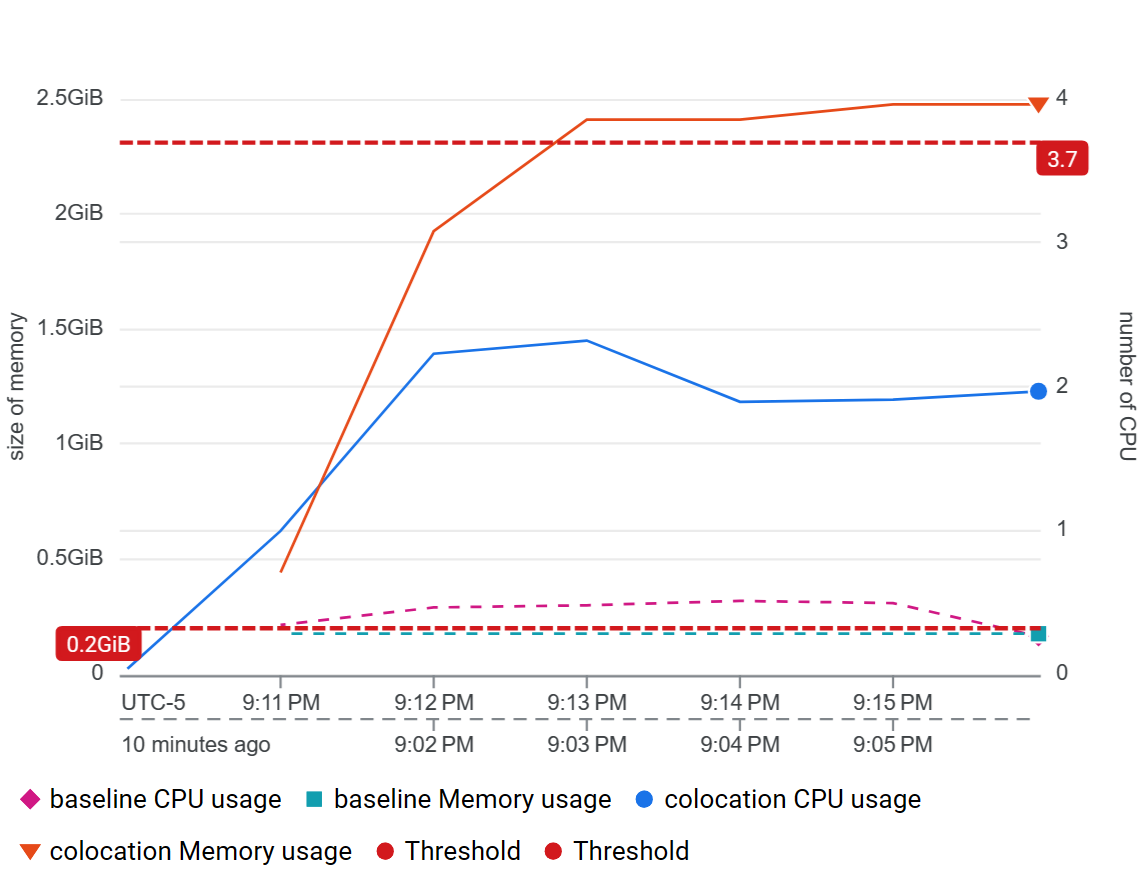
\includegraphics[width=0.5\textwidth]{img-eva-expr1.png}
	\caption{Result for No.3 and No.4 Experiments}
	\label{fig:res-1}
\end{figure}
